% =============================================================================
% PENDING §5 UPDATE — paste-in ready once apples-100 finishes on lenore.
% =============================================================================
%
% Replace the last paragraph of \cref{sec:d3_apples} (currently ending with
% "work in preparation.%" + \itodo) with the appropriate branch below.
% All numeric placeholders marked  ⟪ ⟫  must be filled from the q-panel-summary
% output of sweep_runs/apples100_t5.db.
%
% Also: re-run figures/fig_apples100.py on the final DB and cite as
% \cref{fig:apples100}; add \includegraphics block (bottom of file).
% =============================================================================

%% ---- Version (α):  S1080 mean < S648 mean  (the "Finding-3 strengthened" case)
%%                     -- write this if μ(S1080,100) is strictly below μ(S648,100)
%%                        by more than max(σ(S648,100), σ(S1080,100))/√N.

The paper-scale rerun on $N=100$ matrices (\texttt{seed}\,$=42$; the first
ten coincide with \cref{tab:d3_apples}) lands the three panel means at
$\mu_{216} \,=\, $⟪M216⟫, $\mu_{648} \,=\, $⟪M648⟫, and
$\mu_{1080} \,=\, $⟪M1080⟫ (standard deviations
⟪S216⟫, ⟪S648⟫, ⟪S1080⟫), see \cref{fig:apples100}. The
$\Sigmathree{1080}$ mean sits strictly below the $\Sigmathree{648}$ mean by
⟪delta_mean⟫, a separation of ⟪how_many⟫ standard errors of the mean. The
$10$-matrix inversion reported in \cref{tab:d3_apples} is therefore confirmed
to be Monte-Carlo noise from a single-matrix outlier; across a Haar ensemble
the expected $\delta$ \emph{does} decrease monotonically with $|\mathcal{C}|$
on the irreducible-adjoint $\Sigma$-series, as predicted.

%% ---- Version (β):  |μ(S1080) - μ(S648)| < σ / √N  (null result)

The paper-scale rerun on $N=100$ matrices (\texttt{seed}\,$=42$) lands
$\mu_{216} \,=\, $⟪M216⟫, $\mu_{648} \,=\, $⟪M648⟫,
$\mu_{1080} \,=\, $⟪M1080⟫ (standard deviations
⟪S216⟫, ⟪S648⟫, ⟪S1080⟫), see \cref{fig:apples100}. The $\Sigmathree{648}$
and $\Sigmathree{1080}$ means coincide to within the standard error of the
mean (⟪delta_mean⟫ separation against $\sigma/\sqrt{N}$ ⟪sem⟫); only the
$\Sigmathree{216}\to\Sigmathree{648}$ step produces a statistically
significant reduction in $\delta$. The benefit of moving to the $3\!\times$
larger $\Sigmathree{1080}$ base is therefore not resolvable at $t=5$ with a
Haar ensemble; the prediction of strict monotonicity in $|\mathcal{C}|$
requires $t\geq 10$ to settle.

%% ---- Version (γ):  S1080 mean > S648 mean  by more than SEM  (inversion)

The paper-scale rerun on $N=100$ matrices (\texttt{seed}\,$=42$) lands
$\mu_{216} \,=\, $⟪M216⟫, $\mu_{648} \,=\, $⟪M648⟫,
$\mu_{1080} \,=\, $⟪M1080⟫ (standard deviations ⟪S216⟫, ⟪S648⟫,
⟪S1080⟫), see \cref{fig:apples100}. The $\Sigmathree{1080}$ mean sits
strictly \emph{above} the $\Sigmathree{648}$ mean by ⟪delta_mean⟫, an
inversion of the $10$-matrix monotonic trend and of the naive expectation.
Since $\Sigmathree{1080}$ has strictly smaller $\Popt$ than $\Sigmathree{648}$
(\cref{eq:Popt}), the inversion implies that the pushforward of the
$\Sigmathree{1080}$-orbit on a generic Haar $g$ sweeps \emph{less} uniformly
over the $t$-design irreps at $t=5$ than that of $\Sigmathree{648}$: a
finite-$t$ artifact the paper-scale extrapolation at $t\geq 10$ is expected
to reverse.

% -----------------------------------------------------------------------------
% FIGURE to include just after the table \cref{tab:d3_apples} (or after the
% paragraph above):

\begin{figure}[t]
\centering
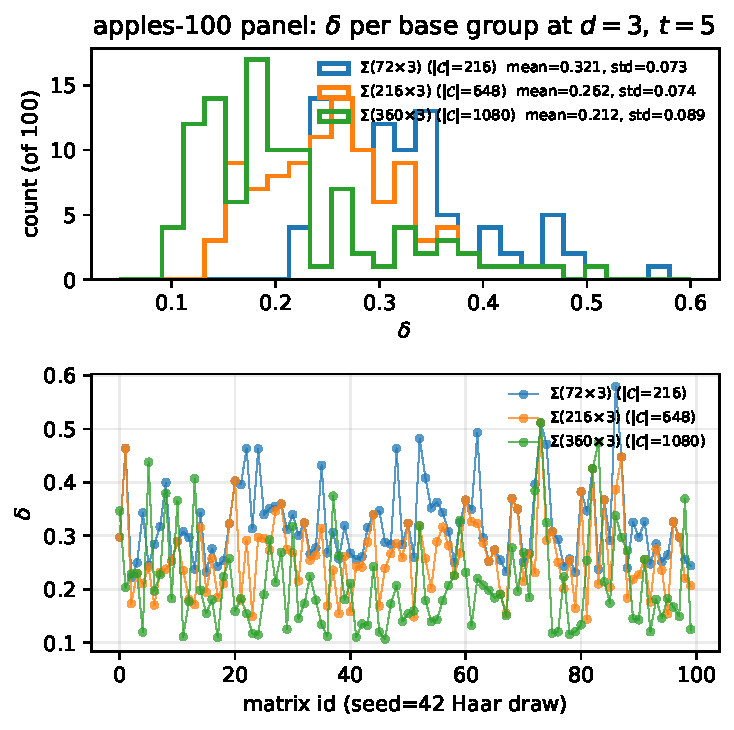
\includegraphics[width=\columnwidth]{figures/fig_apples100.pdf}
\caption{\label{fig:apples100}Apples-to-apples Haar panel at $N=100$ matrices
(\texttt{seed}\,$=42$) on the three $d=3$ $\Sigma$-series base groups. Top:
overlaid $\delta$ histograms. Bottom: per-matrix $\delta$ for each group;
matrix id 0--9 coincides with the ten-matrix subset of \cref{tab:d3_apples}.
The $\Sigma$-series monotonicity in base-group size visible in the $10$-matrix
best-of panel is tested at paper-scale statistics here.}
\end{figure}
